	\documentclass[11pt, a4paper]{article}
\usepackage[margin=2cm]{geometry}
\usepackage{helvet}
\usepackage{graphicx}
\usepackage{lineno}
\usepackage{breakcites}
\usepackage{hyperref}
\graphicspath{ { } }
\renewcommand{\familydefault}{\sfdefault}
\renewcommand{\baselinestretch}{1.5}


\begin{document}
\vspace{20cm}
\title{Ancient Genome Cross-validation of Modelled Selection Co-efficients in Middle-Eastern \& African 		Populations}
\author{Tom Davy [t.davy17@imperial.ac.uk]}	
\maketitle
Main Supervisor: Dr. Jason Hodgson, Imperial College London, j.hodgson@imperial.ac.uk


\begin{figure}
 \centering
\vspace{1cm}

\includegraphics[scale=0.13]{Imperial.png}
\end{figure}


\pagebreak
\linenumbers

Key Words: Human Evolution, Selection, Introgression, Population Genetics, Ancient DNA
%\vspace{0cm}
\section{Project Introduction}
The first currently surviving human population lineages to have left Africa would have been exposed to an entire suite of environmental pressures in the form of changes to diet, ecosystem \& pathogenic landscape, all of which would have acted upon the genomic landscape of these migratory populations, possibly selecting for certain variants from background variation or novel mutation. 

Recent analyses \cite{Gresham2017} have demonstrated that populations in the Middle-East (ME), after suitable time for a selective process to occur, had the opportunity to admix with African populations, leading to both populations experiencing admixture and conserving a quantifiable amount of introgressed genetic content. Applications of the LSBL test has suggested that such tracts may be under selective pressure, and an overlap in the candidate loci for selection between these populations are under selection within both populations, suggesting that admixture can function as an adaptive event at the population level. In this project, I aim to delineate these selection co-efficients via modelling the population history of these allele frequencies, then applying this workflow to a real dataset consisting of SNPs for 259,257 SNPs from across several African populations \cite{Hodgson2014}.

\begin{sloppypar}
Importantly, recent publication of ancient African genomes \cite{Skoglund2017, llorente2015ancient} may allow us to validate my Selection co-efficient predictions through time using real empirical data.
\end{sloppypar}
	
			
	\section{Proposed Methodology}
Firstly, a simulation of the experimental framework will be conducted with forward simulations through SFS-code \cite{Hernandez2008}. Ancestral and admixed populations, upon which selection would have acted on sites of introgression as seen in \cite{Gresham2017} will be scored using the adapted locus-specific branch length (LSBL) test \cite{Gresham2017}, which can be leveraged to predict selection-co-efficient as a function of daughter population branch width. Presence or absense of predicted genotypes in the admixed  across the ancestral population genomes will then be scored for correct predictions, giving us a metric against which to validate this process. Model fitting of differing simulation parameters will be performed via a log-likelihood ratio approach. Simulated VCF files will also be verified in Plink \cite{Chang2015} via the pair-wise F-statistic before downstream analyses. 

The Horn of Africa \& Middle Eastern Genomic datasets from the 260k SNP dataset \cite{Hodgson2014} will then be similarly utilised via this method. Presence or absense of predicted genotypes across the ancient genomes will then be scored for correct predictions, where a null population is direct mapping of current allelic frequencies to the ancient genome, giving us a metric against which to validate this process. The Mota man \cite{llorente2015ancient} will also be investigated via the adapted LSBL test to these analyses to identify presence of abscense of introgression, which is important in terms of intepreting predicting selection co-efficients across this ancient genome.

	\section{Anticipated Outcomes and Outputs}
	This project aims to input into a manuscript of high research-impact upon completion. 
	
	
	
	\section{Project Feasibility}
	
	
	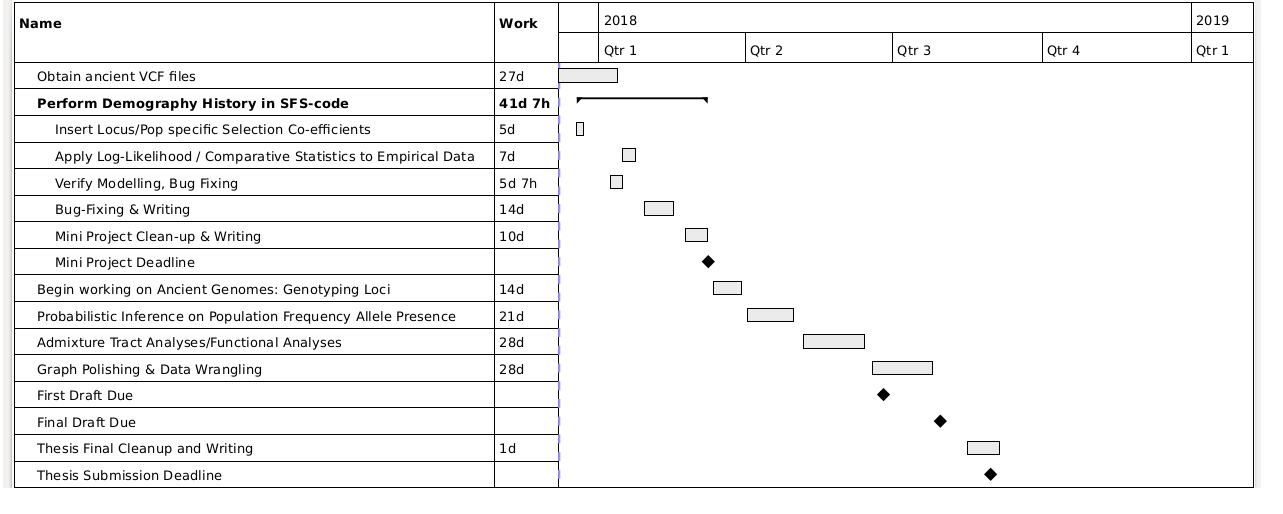
\includegraphics[scale=1.5]{Gantt.png} 



	\section{Budget}

Being purely computational, budget can be put towards the attendance of relevant meetings, such as to present and discuss such work. Candidates include ESHE 2018  \url{http://www.eshe.eu/meetings.html} A presumptial budget for attendance at this meeting follows. 

\begin{table}[ht]
\caption{ESHE 2018 Attendance Budget}
\centering
\begin{tabular}{c c}
\hline
Item & Cost(GBP) \\ [0.5ex]
\hline
Transport & 163.00			\\
Registration & 44.00	\\
Accomodation & 150.00	\\
Poster Printing & 15.00 \\
\hline
Total & 373.00			\\ [1ex]
\hline
\end{tabular}
\end{table}

\pagebreak

\bibliographystyle{apalike}
\bibliography{Proposal}


\pagebreak	
 
 

\begin{center}

\section{Supervisor Budgetary Approval}


\vspace{2cm}
\textit
{"I have seen and approved the proposal and the budget"}
\vspace{1cm}


\includegraphics[scale=0.4]{JHsig.png}


Jason A. Hodgson \linebreak
8/10/17

\end{center}
\end{document}


